\chapter{In Progress}
\label{chapter:in_progress}

\section{Deliverables}

\begin{itemize}

\item{\bf D-3 - Requirements Baseline Document}

Planning of the structure and content of the requirements baseline document has begun.

\item{\bf D-16 - Level 1 Review Technical Note}

A technical note describing the Odin/SMR calibration
routine, radiometric performance, and Level1 data is under production (WP 1.1.3). 
      

\end{itemize}


\section{Work Packages}

\begin{itemize}

\item{\bf WP 1.1.1.3 - Compare with Simulated Data}

This work package aims to compare the measured brightness temperature in the level1b data with brightness temperature simulated with ARTS. The work investigates frequency modes 1 and 2. Measurements from low tangent altitudes result in a flat spectrum, as the satellites essentially receives black body radiation at tangent altitudes below 8km for FM 1, and 10km for FM 2. The investigations use conditions in which the atmosphere is relatively isothermal between 10-15 km, since the atmosphere becomes optically dense at approximately that range, and the measured spectrum should be independent of the exact height from which the radiation originates. These conditions occur most likely during June-July for the latitudes 60N-90N and during January-February for the latitudes 60S-90S. Therefore, these periods constitute the investigated months investigated for each hemisphere between the years 2002-2014. We carried out investigations for both the northern and southern hemispheres for FM 1 and 2. ERA-Interim temperature profiles comprise the temperature profiles used for simulations.

Figure \ref{fig:Measured_simulated} shows an example of a measured and simulated spectrum for FM 2. We use the mean value of the flat part of the simulated and the measured spectrum to calculate the error between the two. The median error of all spectra within one year constitutes the error used to compare the error between individual years. Figure \ref{fig:Error} shows the error between the simulated and measured spectra for FM 1 in the northern hemisphere. A negative value indicates that the simulated brightness temperature exceeds that of the measured spectrum. The error bars describe the uncertainty of the median error. Figure \ref{fig:Error} suggests that the error  is predominantly negative with maximum positive and negative errors and 0.2K and -1K respectively. Furthermore, the measured and simulated brightness temperatures can be investigated separately. In FM 1 in the northern hemisphere, the median of the measured brightness temperature varies between 214.8K and 216.6K. The median of the simulated brightness temperature varies between 215K and 216.6K. Both values seem stable although Figure \ref{fig:Error} does suggest a systematic negative error.

Additionally, we analyse the southern hemisphere of FM 1 as well as both hemispheres for FM 2 to investigate the stability of the measured and simulated brightness temperatures. So far results suggest that the median measured brightness temperature for FM 1 decreases a maximum of 1K between 2002-2014. The median measured brightness temperature for FM 2 decreases almost 4K in the northern hemisphere, but only 1K in the southern hemisphere between 2002-2014. Simulated brightness temperatures are stable for all cases with a slight increasing trend in the southern hemisphere (0.5K-1K between 2002-2014).

\begin{figure}[b]
\centering
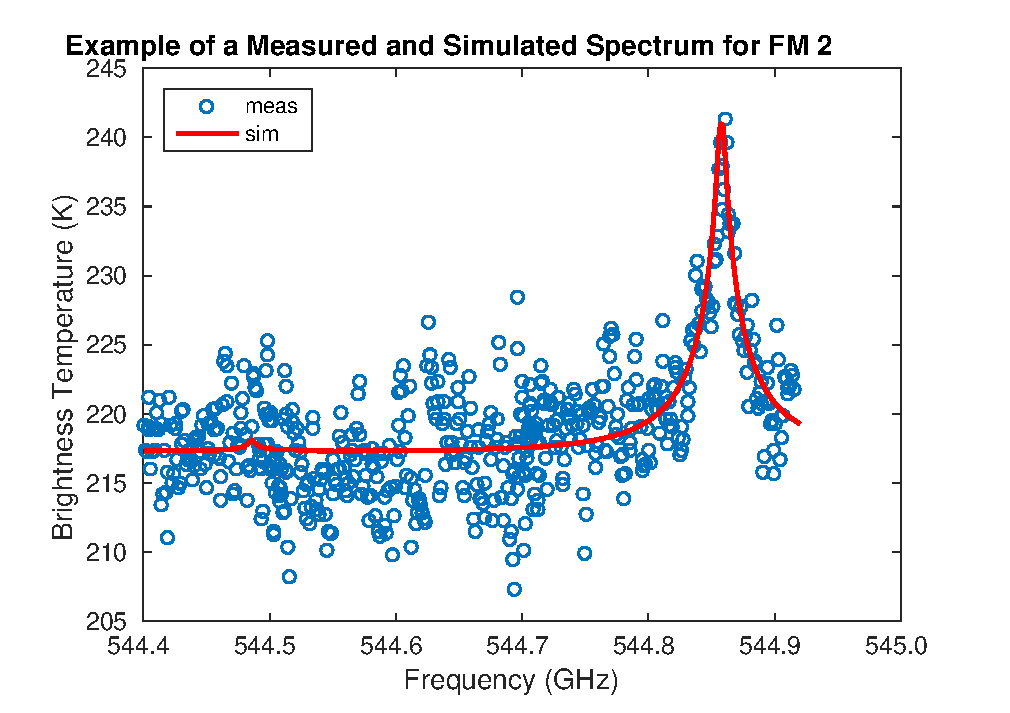
\includegraphics[scale = 0.7]{figures/fm2.eps}
\caption{Measured and simulated spectrum for FM 2}
\label{fig:Measured_simulated}
\end{figure}


\begin{figure}[t]
\centering
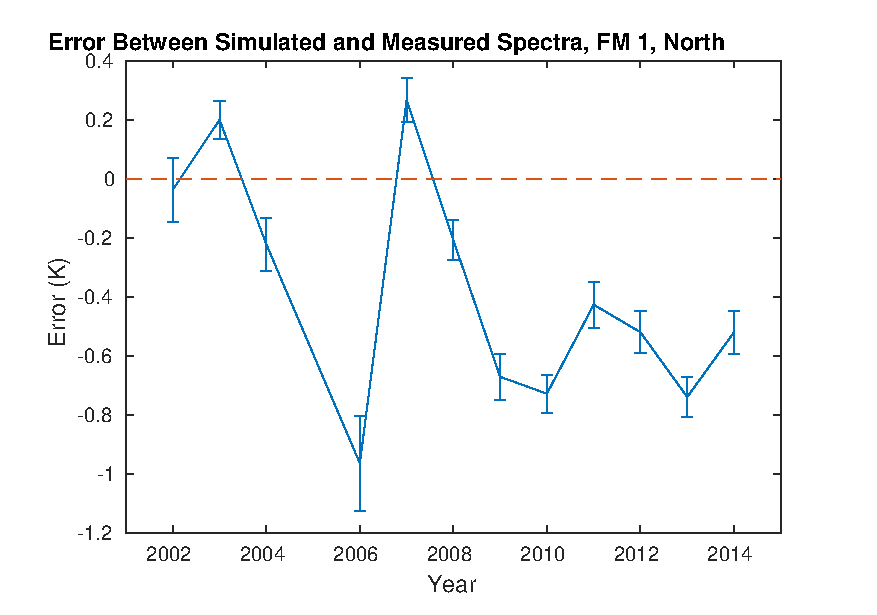
\includegraphics[scale = 0.8]{figures/Error_fm1_n.eps}
\caption{Error between the simulated and measured spectra for FM 1 in the northern hemisphere}
\label{fig:Error}
\end{figure}


\item{\bf WP 1.1.2.3 Comparison of Calibration Versions}

This WP deals with comparison of calibration version 7 (v.7) and 8 (v.8) data. 
v.8 builds upon v.7 calibration routine, but is extended and more advanced.
v.8 is scan-based whereas v.7 is orbit based, and v.8 aims to remove ripples
seen in the spectra in the upper part of the scan in the v.7 data.

Production of comparison plots of data from the two versions is ongoing.
On many occasions the data from the two versions differs only marginally,
but v.7 data clearly shows better performance for measurements
in the upper part of scan.

\item{\bf WP 1.1.3 - Technical Note}

Production of a technical note describing the Odin/SMR calibration
routine, radiometric performance, and Level1 data is ongoing.

\item{\bf WP 2.1.3 - Write Requirements Baseline Document (RB)}

Planning of the structure and content of the RB document has begun.

\end{itemize}
